% Preamble
\documentclass[twocolumn, linenumbers, twocolappendix]{aastex631}
%\documentclass[twocolumn]{aastex631}
\usepackage{natbib}
\usepackage{latexsym}
\usepackage{graphicx}
\usepackage{epsfig}
\usepackage{amssymb}
\usepackage{amsmath}
\usepackage{epstopdf}
\usepackage{hyperref}
\usepackage{xcolor}

%%%% Custom commands
\newcommand{\yL}{\ensuremath{\mathcal{Y}_{\rm{L}}}}
\newcommand{\yS}{\ensuremath{\mathcal{Y}_{\rm{S}}}}
\newcommand{\justgrad}{\ensuremath{\nabla}}
\newcommand{\gradrad}{\ensuremath{\nabla_{\rm{rad}}}}
\newcommand{\gradad}{\ensuremath{\nabla_{\rm{ad}}}}
\newcommand{\gradC}{\ensuremath{\nabla_{\mathrm{C}}}}
\newcommand{\gradmu}{\ensuremath{\nabla_{\mu}}}
\newcommand{\gradL}{\ensuremath{\nabla_{\mathrm{L}}}}
\newcommand{\gradT}{\ensuremath{\nabla_{\mathrm{T}}}}
\newcommand{\Ro}{\ensuremath{\mathrm{R}_{0}}}
\newcommand{\delp}{\ensuremath{\delta_{\rm{p}}}}
\newcommand{\Fbot}{\ensuremath{F_{\rm{bot}}}}
\newcommand{\Ftot}{\ensuremath{F_{\rm{tot}}}}
\newcommand{\Frad}{\ensuremath{F_{\rm{rad}}}}
\newcommand{\Fconv}{\ensuremath{F_{\rm{conv}}}}
\newcommand{\Fcz}{\ensuremath{F_{\rm{cz}}}}
\newcommand{\mP}{\ensuremath{\mathcal{P}}}
\newcommand{\mD}{\ensuremath{\mathcal{D}}}
\newcommand{\dP}{\ensuremath{\delta_{\rm{p}}}}
\newcommand{\Lcz}{\ensuremath{L_{\rm{CZ}}}}
\newcommand{\mR}{\ensuremath{\mathcal{R}}}
\newcommand{\mS}{\ensuremath{\mathcal{S}}}
\newcommand\Pran{\ensuremath{\mathrm{Pr}}}
\newcommand{\brunt}{{Brunt--V\"{a}is\"{a}l\"{a}}}

\newcommand{\angles}[1]{\langle #1 \rangle}
\newcommand{\pd}[1]{\partial_{#1}}
\renewcommand{\vec}[1]{\boldsymbol{#1}}
\newcommand{\M}[1]{\mathbf{#1}}
\renewcommand{\dot}{\vec{\cdot}}
\renewcommand{\bar}[1]{\overline{#1}}
\newcommand{\grad}{\vec{\nabla}}
\newcommand{\cross}{\vec{\times}}
\newcommand{\laplacian}{\nabla^2}

\newcommand{\editone}[1]{\textcolor{orange}{#1}}

\newcommand{\todo}[1]{ {\color{blue} \noindent\footnotesize \\\textsf{}TODO:} \textsf{#1}\\\noindent }


%%%% Journal preamble
\received{}
\revised{}
\accepted{}
\published{}
\submitjournal{ApJ}

\shorttitle{Schwarzschild or Ledoux}
\shortauthors{Anders et al}


\begin{document}

%%%% Title and Abstract
\title{Schwarzschild and Ledoux are equivalent on evolutionary timescales}
\author[0000-0002-3433-4733]{Evan H. Anders}
\affiliation{CIERA, Northwestern University, Evanston IL 60201, USA}
\affiliation{Kavli Institute for Theoretical Physics, University of California, Santa Barbara, CA 93106, USA}
\author[0000-0001-5048-9973]{Adam S. Jermyn}
\affiliation{Center for Computational Astrophysics, Flatiron Institute, New York, NY 10010, USA}
\affiliation{Kavli Institute for Theoretical Physics, University of California, Santa Barbara, CA 93106, USA}
\author[0000-0002-7635-9728]{Daniel Lecoanet}
\affiliation{CIERA, Northwestern University, Evanston IL 60201, USA}
\affiliation{Department of Engineering Sciences and Applied Mathematics, Northwestern University, Evanston IL 60208, USA}
\affiliation{Kavli Institute for Theoretical Physics, University of California, Santa Barbara, CA 93106, USA}
\author[0000-0003-4323-2082]{Adrian E. Fraser}
\affiliation{Department of Applied Mathematics, Baskin School of Engineering, University of California, Santa Cruz, Santa Cruz, CA 95064, USA}
\affiliation{Kavli Institute for Theoretical Physics, University of California, Santa Barbara, CA 93106, USA}
\author[0000-0002-4538-7320]{Imogen G. Cresswell}
\affiliation{Department Astrophysical and Planetary Sciences \& LASP, University of Colorado, Boulder, CO 80309, USA}
\affiliation{Kavli Institute for Theoretical Physics, University of California, Santa Barbara, CA 93106, USA}
\author[0000-0003-2124-9764]{J. R. Fuentes}
\affiliation{Department of Physics and McGill Space Institute, McGill University, 3600 rue University, Montreal, QC H3A 2T8, Canada}

\correspondingauthor{Evan H. Anders}
\email{evan.anders@northwestern.edu}

\begin{abstract}
    In one-dimensional stellar evolution models, convective boundaries are calculated using either the Schwarzschild or Ledoux criterion, but there is no consensus regarding which criterion to use.
    In this letter, we present a 3D hydrodynamical simulation of a convection zone and adjacent radiative zone, including both thermal and compositional buoyancy forces.
    As expected, regions which are unstable according to the Ledoux criterion are convective.
    Initially, the radiative zone adjacent to the convection zone is Schwarzschild-unstable but Ledoux-stable due to a composition gradient.
    Over many convective overturn timescales the convection zone grows via entrainment.
    The convection zone saturates at the size predicted by the Schwarzchild criterion, and in this final state the Schwarzschild and Ledoux criteria are equivalent.
    Therefore, the size of stellar convection zones is determined by the Schwarzschild criterion, except possibly during short-lived stages in which entrainment persists.
\end{abstract}
\keywords{Stellar convection zones (301), Stellar physics (1621); Stellar evolutionary models (2046)}



%%%% Body of paper

\section{Introduction}
\label{sec:introduction}
Observations tell us that we do not understand the positioning of convective boundaries in stars.
For example, models and observations disagree about the sizes of convective cores \citep{claret_torres_2018, viani_basu_2020, pedersen_etal_2021, johnston_2021}, lithium abundances in solar-type stars \citep{pinsonneault_1997, sestito_randich_2005, carlos_etal_2019, dumont_etal_2021}, and the sound speed at the base of the Sun's convection zone \citep[see][Sec.~7.2.1]{basu_2016}.
Improperly estimating convective boundary locations can have important impacts across astrophysics such as by affecting the mass of stellar remnants \citep{farmer_etal_2019, mehta_etal_2022} and the inferred radii of exoplanets \citep{basu_etal_2012, morrell_2020}.

While convective boundary mixing (CBM) has many uncertainties, the most fundamental question is: what determines the location of convection zone boundaries? 
Some authors evaluate the \emph{Schwarzschild criterion}, which determines where the temperature and pressure stratification within a star are stable or unstable.
Others evaluate the \emph{Ledoux criterion}, which accounts for stability or instability due to compositional stratification \citep[e.g., the variation of helium abundance with pressure; see][chapter 3, which reviews these criteria]{salaris_cassisi_2017}.
Recent authors state that these criteria should be equivalent at a convective boundary according to mixing length theory \citep{gabriel_etal_2014, mesa4, mesa5}, but in practice these criteria are often different at convective boundaries in stellar evolution software instruments, and a variety of workarounds have been proposed to address this~\citep{mesa4,mesa5}.

There is still disagreement regarding which stability criterion to employ~\citep[discussed in][chapter 2]{kaiser_etal_2020}.
Multi-dimensional simulations show that convection zones with Ledoux-stable boundaries expand by entraining compositionally-stable regions \citep{meakin_arnett_2007, woodward_etal_2015, jones_etal_2017, cristini_etal_2019, fuentes_cumming_2020, andrassy_etal_2020, andrassy_etal_2021}.
It is unclear from past 3D simulations whether that entrainment should stop, leading to uncertainty in how to include entrainment in 1D models \citep{staritsin_2013, scott_etal_2021}.

In this letter, we present a simple 3D hydrodynamical simulation that demonstrates that convection zones with Ledoux-stable but Schwarzschild-unstable boundaries entrain material until the Ledoux and Schwarzschild criteria agree on the location of the convective boundary.
Therefore, in 1D stellar evolution models, when evolutionary timescales are much larger than the convective overturn timescale \citep[such as on the main sequence, see][]{georgy_etal_2021}, the Schwarzschild criterion describes the location of the convective boundary, and Ledoux and Schwarzschild should agree if properly implemented.
We discuss these criteria in Sec.~\ref{sec:theory}, display simulations in Sec.~\ref{sec:results}, and briefly discuss in Sec.~\ref{sec:conclusions}.


\begin{figure*}[t!]
\centering
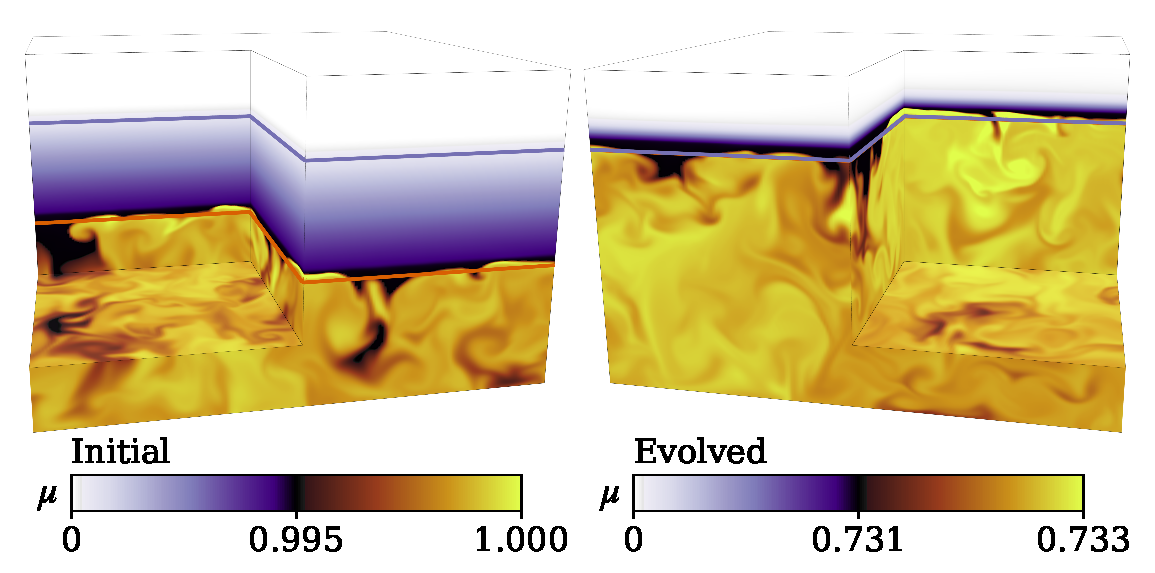
\includegraphics[width=\textwidth]{dynamics_figure.pdf}
\caption{
    Volume renderings of the composition $\mu$ at early (left) and late (right) times.
    The change in color from white at the top of the box to dark purple at the top of the convection zone denotes a stable composition gradient.
    The convection zone is well-mixed, so we expand the colorbar scaling there; black represents entrained low-$\mu$ fluid being mixed into the yellow high-$\mu$ convection zone.
    The orange and purple horizontal lines respectively denote the heights at which $\yL = 0$ and $\yS = 0$.
    The two criteria are equivalent in the right panel, so the orange line is not visible.
    The simulation domain spans $z \in [0, 3]$, but we only plot $z \in [0, 2.5]$ here.
\label{fig:dynamics}
}
\end{figure*}

\section{Theory \& Experiment}
\label{sec:theory}
Convective stability can be determined using the Schwarzschild criterion,
\begin{equation}
    \yS \equiv \gradrad - \gradad,
    \label{eqn:yS}
\end{equation}
or the Ledoux criterion,
\begin{equation}
    \yL \equiv \yS +  \frac{\chi_\mu}{\chi_T}\gradmu.
    \label{eqn:yL}
\end{equation}
The temperature gradient $\justgrad \equiv d \ln P / d \ln T$ (pressure $P$ and temperature $T$) is $\gradad$ for an adiabatic stratification and $\gradrad$ if the flux is entirely carried radiatively.
The composition gradient $\gradmu = d\ln\mu/d\ln P$ (mean molecular weight $\mu$) is modified by $\chi_T = (d\ln P / d\ln T)_{\rho,\mu}$ and $\chi_\mu = (d\ln P / d\ln\mu)_{\rho,T}$ (density $\rho$).

In Eqns.~\ref{eqn:yS} and \ref{eqn:yL}, $\mathcal{Y}$ is the discriminant \citep[e.g.,][sec.~2]{mesa4}, which is like the superadiabaticity.
Stellar structure codes assume that convective boundaries coincide with the root (sign change) of the discriminant.
The various stability regimes which can occur in stars are described in section 3 and figure 3 of \citet{salaris_cassisi_2017}, but note four important regimes:
\begin{enumerate}
    \item Convection Zones (CZs): Regions with $\yS > 0$ and $\yL \geq \yS$ are convectively unstable.
    \item Radiative Zones (RZs): Regions with $\yS < 0$ and $\yL \leq \yS$ are stable to convection.
    \item ``Semiconvection'' Zones (SZs): Regions with $\yS > 0$ but $\yL < 0$ are stablized to convection by a composition gradient despite an unstable thermal stratification.
        These regions can be stable RZs or linearly unstable to overstable doubly diffusive convection \citep[ODDC, see][chapter 2]{garaud_2018}.
    \item ``Thermohaline'' Zones: Regions with $\yS < 0$ and $\yL > \yS$ are thermally stable to convection despite an unstable composition gradient.
        These regions can be stable RZs or linearly unstable to thermohaline mixing \citep[see][chapter 3]{garaud_2018}.
\end{enumerate}
In this paper, we study 3D simulations of a stable SZ (\#3) bounded below by a CZ (\#1) and above by an RZ (\#2).
We examine how the boundary of the CZ evolves through entrainment.
In particular, we are interested in seeing if the roots of $\yS$ and $\yL$ coincide after evolution.
%Since stellar evolution timesteps generally span many convective overturn times, our 3D simulation should evolve to the proper state, which may be quite different from our initial conditions.

In this work, we utilize a simplified 3D model which employs the Boussinesq approximation, which assumes that the depth of the layer being studied is much smaller than the local scale height.
Since we are studying thin regions near convective boundaries, this assumption is OK.
The relevant physics for this problem are included ($\gradrad$ varies with height, buoyancy is determined both by the composition $\mu$ and the temperature stratification $T$), so $\yS$ and $\yL$ are meaningfuly defined and distinct from one another when composition gradients are present.
For details on our model setup and Dedalus simulations, we refer the reader to appendices \ref{app:model} and \ref{app:simulation_details}.


\begin{figure*}[t]
\centering
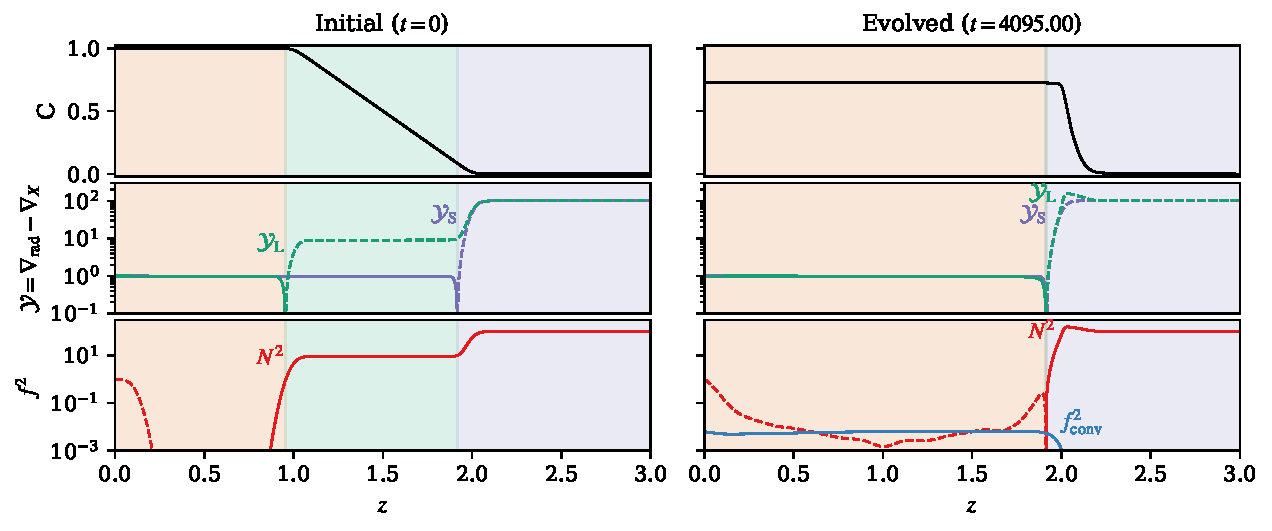
\includegraphics[width=\textwidth]{fig2_profiles.pdf}
\caption{
    Horizontally-averaged profiles of the composition (top), the discriminants $\yS$ and $\yL$ (middle, Eqns.~\ref{eqn:yS} \& \ref{eqn:yL}), and the \brunt$\,$ frequency $N^2 = -\yL$ and the square convective frequency $f_{\rm{conv}}^2$ (bottom, Eqn.~\ref{eqn:fconv2}).
    Positive and negative values are respectively solid and dashed lines.
    We show the initial (left) and evolved (right, time-averaged over 100 convective overturn times) states.
    There are no motions in the initial state, so $f_{\rm{conv}}^2 = 0$ and does not appear.
    The background color is orange in CZs, green in SZs, and purple in RZs per Section ~\ref{sec:theory}.
    The lightly hashed background region in the evolved RZ is the mechanical overshoot zone.
\label{fig:profiles}
}
\end{figure*}



\section{Results}
\label{sec:results}

Fig.~\ref{fig:dynamics} visualizes the composition field in our simulation near the initial state (left) and evolved state (right).
Overplotted horizontal lines correspond to the roots of $\yL$ (orange, Ledoux boundary) and $\yS$ (purple, Schwarzschild boundary).
Initially, the bottom third of the domain is a CZ, the middle third is an SZ, and the top third is an RZ.
Convection mechanically overshoots at all times, which can be seen by the presence of convection a small but appreciable distance above the orange Ledoux boundary.
Overshoot occurs because the Ledoux boundary corresponds to the sign change in the buoyant acceleration, not where the convective velocity is zero.

The most obvious change from the left to the right panel is that the CZ has consumed the SZ and fills the bottom two-thirds of the box.
The overshooting convective motions entrained low-composition material from above the Ledoux boundary into the CZ.
Convective motions mixed this fluid, and this process repeated over thousands of convective overturn times until the Ledoux and Schwarzschild boundaries of the CZ coincided.
After becoming Schwarzschild stable, the convective boundary stopped moving.
This occurs because the radiative flux renews and reinforces the radiative gradient, but there is no equivalent process for the composition.

Figure \ref{fig:profiles} displays vertical simulation profiles in the initial (left) and evolved (right) states.
Shown are the composition $\mu$ (top), the discriminants $\yL$ and $\yS$ (middle), and the square \brunt$\,$ frequency (top) as well as the square convective frequency defined as
\begin{equation}
f_{\rm{conv}}^2 = \frac{|\vec{u}|^2}{\ell_{\rm{conv}}^2},
\label{eqn:fconv2}
\end{equation}
where $\vec{u}$ is the velocity and $\ell_{\rm{conv}}$ is the depth of the convectively unstable layer.

Initially, the composition is uniform in the CZ ($z < 1$) and RZ ($z > 2$), but varies linearly in the SZ ($z \in [1, 2]$).
The root of $\yL$ occurs at $z \approx 1$ while that of $\yS$ occurs at $z \approx 2$.
Furthermore, $f_{\rm{conv}}^2 = 0$ in the initial, stationary state.
The \brunt$\,$ frequency $N^2$ is negative in a boundary layer at the base of the CZ which drives the instability.
$N^2$ is stable for $z \gtrsim 1$, and is larger in the RZ than the SZ by an order of magnitude\footnote{We ran simulations where $N^2$ was identical in the RZ and SZ and saw similar behavior.
We make $N^2$ large in the RZ to reduce overshoot and wave mixing in the evolved state.}

The evolved state is attained after convection entrains and mixes the stabilizing fluid in the SZ.
We see that the composition profile (top) is constant in the CZ and overshoot zone (denoted as a transparent hashed region), but approximates a step function at the top of the overshoot zone.
The roots of the discriminants $\yL$ and $\yS$ coincide (middle).
Furthermore, in the CZ, the convective frequency is roughly constant and $N^2 \lesssim 0$ (bottom).
In the RZ, $f_{\rm{conv}}^2 \approx 0$ and $N^2 \gg 0$.
We can compute the ``stiffness'' of the radiative-convective interface,
\begin{equation}
\mS = \frac{N^2|_{\rm{RZ}}}{f_{\rm{conv}}^2|_{\rm{CZ}}},
\label{eqn:stiffness}
\end{equation}
which is related to the oft-studied Richardson number.
In our evolved simulation, we measure $\mS \sim 10^{4}$.
Boundaries with a low stiffness $\mS \lesssim 10$ easily deform in the presence of convective flows, but convective boundaries in stars often have $\mS \gtrsim 10^6$.
The number of convective overturn times required to entrain the SZ scale with $\mS$; we have chosen to use a large value of $\mS$ here to ensure our simulations are in the right regime to study entrainment at a stellar convective boundary.

Finally, Figure \ref{fig:kippenhahn} displays a Kippenhahn-like diagram of the simulation's height vs.~time to show evolutionary trends.
The roots of $\yL$ and $\yS$ are respectively shown as orange (Ledoux boundary) and purple (Schwarzschild boundary) lines.
The CZ is colored orange and sits below the Ledoux boundary, the RZ is colored purple and sits above the Schwarzschild boundary, and the SZ is colored green and is between these boundaries.
Convection motions overshoot above the Ledoux boundary.
The height where the horizontally-averaged kinetic energy falls below 10\% of its bulk-CZ value is marked with a black line, and the hashed region below it is the overshoot zone.
We note that the black line and overshoot zone roughly correspond with the maximum of $\partial\mu/\partial z$ (Fig.~\ref{fig:profiles}, upper right), so this describes overshoot well.
Importantly, note that the Schwarzschild and Ledoux boundaries start at different heights, but 3D convective mixing causes them to converge on dynamical timescales.




\begin{figure}[t!]
\centering
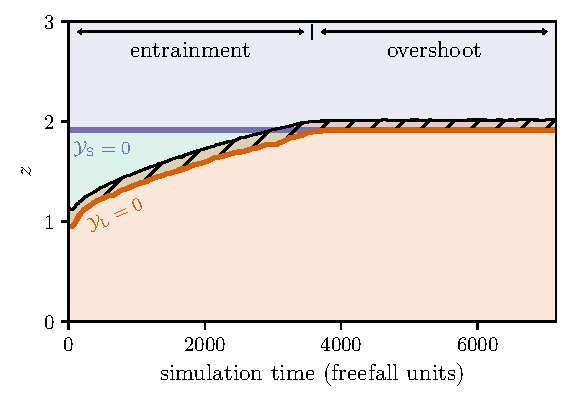
\includegraphics[width=\columnwidth]{kippenhahn.pdf}
\caption{
    A Kippenhahn-like diagram of the simulation evolution.
    The $y$-axis is simulation height and the $x$-axis is simulation time.
    The orange line denotes the convective boundary according to the Ledoux criterion ($\yL = 0$); the CZ is below this and is colored orange.
    The purple line denotes the convective boundary according to the Schwarzschild criterion ($\yS = 0$); the RZ is above this and is colored purple.
    The semiconvective region between these boundaries is colored green.
    The overshoot zone is hashed, and the black line denotes the top of this region.
    The simulation has an ``entrainment phase'' while the CZ expands, and a pure ``overshoot phase'' where the convective boundary does not advance.
    {\color{blue} Note: The simulation has only evolved to $t = 17000$, and I extended the end of this; it is running to 20000.}
\label{fig:kippenhahn}
}
\end{figure}


\section{Conclusions \& Discussion}
\label{sec:conclusions}

In this letter, we present 3D simulations of a convection zone and its boundary.
The initial boundary is compositionally stable but weakly thermally unstable (Ledoux stable but Schwarzschild unstable).
Entrainment causes the convective boundary to advance until the Ledoux and Schwarzschild criterion agree upon the location of the convective boundary.

These simulations demonstrate that the Ledoux criterion properly defines the \emph{instantaneous} criterion for the boundary of a convection zone.
However, when the evolutionary timescale $t_{\rm{evolution}} \gg t_{\rm{conv}}$, the convective overturn timescale, the Schwarzschild criterion provides the best description of the steady-state boundary of the convection zone.
Our 3D dynamical simulations support the claim that ``logically consistent'' implementations of mixing length theory \citep{gabriel_etal_2014, mesa4, mesa5} must set the Schwarzschild discriminant $\yS = 0$ at the convective boundary.
This suggests that the MESA software instrument's modern ``convective pre-mixing'' (CPM) algorithm should properly find the boundary of most convection zones.
Put differently, our simulations suggest that 1D stellar evolution models should not produce different answers when using the Schwarzschild or Ledoux criterion for convective stability when $t_{\rm{evolution}} \gg t_{\rm{conv}}$.

We note briefly that many Ledoux-stable but Schwarzschild-unstable regions in stars are unstable to overstable doubly-diffusive convection (ODDC).
ODDC generally mixes more quickly than the entrainment studied here, and has been studied extensively in local simulations \citep{mirouh_etal_2012, wood_etal_2013, xie_etal_2017}; see \citet{garaud_2018} for a nice review.
ODDC has been applied in 1D stellar evolution models to the regions near main sequence stellar convective cores in \citet{moore_garaud_2016}.
They find rapid mixing of ledoux-stable but schwarzschild-unstable regions, and ODDC formulations should should be widely included in stellar models.

For stages in stellar evolution where $t_{\rm{conv}} \sim t_{\rm{evolution}}$, implementations of time-dependent convection \citep[TDC, e.g.,][]{tdc_1986} should be employed to properly capture convective dynamics and the advancement of convective boundaries.
The advancement of convective boundaries in TDC implementations should be informed by time-dependent theories and simulations of the motion of convective boundaries \citep[e.g.,][]{turner_1968, fuentes_cumming_2020}.

The purpose of this study was to understand how the root of the discriminant $\yL$ evolves over time, and whether it coincides with the root of $\yS$ at late times.
While there is interesting behavior near the boundary beyond that point (e.g., mechanical convective overshoot), a detailed analysis of that phenomenon is beyond the scope of this work.
We furthermore constructed the simulations in this work to have a small penetration parameter $\mathcal{P}$ \citep{anders_et_al_2021} and we see negliglble convective penetration in our simulations.
Finally, in our simulations, the radiative conductivity is independent of the magnitude of the composition $\mu$, but this is not the case in stars.
Since the radiative conductivity sets the location of the Schwarzschild boundary, including these effects would change the exact location of our final convective boundary, but would not change the fundamental takeaways of this work.

In summary, we find that the Schwarzschild criterion provides the location of the convective boundary in a statistically stationary state; in this final state, the Ledoux and Schwarzschild criteria are degenerate.


\begin{acknowledgments}
We thank Meridith Joyce, Anne Thoul, Dominic Bowman, Jared Goldberg, Tim Cunningham, Falk Herwig, Kyle Augustson, (OTHERS?) for useful discussions which helped improve our understanding.
EHA is funded as a CIERA Postdoctoral fellow and would like to thank CIERA and Northwestern University. 
AEF acknowledges support from NSF Grant Nos.~AST-1814327 and AST-1908338. 
This research was supported in part by the National Science Foundation under Grant No. PHY-1748958, and we acknowledge the hospitality of KITP during the Probes of Transport in Stars Program.
Computations were conducted with support from the NASA High End Computing (HEC) Program through the NASA Advanced Supercomputing (NAS) Division at Ames Research Center on Pleiades with allocation GID s2276.
The Flatiron Institute is supported by the Simons Foundation.
\end{acknowledgments}


\appendix

\section{Model \& Initial Conditions}
\label{app:model}
In this work we study the simplest possible system: incompressible, Boussinesq convection with a composition field and a height-varying background radiative conductivity, similar to that used in \citet{fuentes_cumming_2020, anders_etal_2022}.
These equations are
\begin{align}
    &\grad\dot\vec{u} = 0
        \label{eqn:incompressible_dimensional}, \\
    &\partial_t \vec{u}\dot\grad\vec{u} = -\frac{1}{\rho_0}\grad p + \frac{\rho_1}{\rho_0}\vec{g} + \nu\grad^2\vec{u}
        \label{eqn:momentum_dimensional}, \\
    &\partial_t T + \vec{u}\dot\grad T + w\gradad + \grad\dot[-\kappa_{T,0}\grad\bar{T}] = \kappa_T\grad^2 T'
        \label{eqn:temperature_dimensional}, \\
    &\partial_t C + \vec{u}\dot\grad C = \kappa_{C,0}\grad^2\bar{C} + \kappa_C\grad^2 C'
        \label{eqn:composition_dimensional}, \\
    &\frac{\rho_1}{\rho_0} = -|\alpha|T + |\beta|C
        \label{eqn:boussinesq}.
\end{align}
Here, $\vec{u}$ is the vector velocity, $T$ is the temperature, $C$ is the composition, $\rho_0$ is the constant background density, $\p$ is the kinematic pressure which enforces Eqn.~\ref{eqn:incompressible_dimensional}, $\rho_1$ are density fluctuations which act only on the buoyant term, and $\alpha$ and $\beta$ are the thermal and compositional expansion coefficients, and $\gradad$ is the adiabatic gradient.
Diffusive terms are controlled by the kinematic viscosity $\nu$, as well as the thermal diffusivity $\kappa_T$ and compositional diffusivity $\kappa_C$.
On the horizontally-invariant ($n_x = 0$ and $n_y = 0$) mode, we use a height-depended thermal diffusion coefficient $\kappa_{T,0}$ (which allows $\gradrad$ to vary with height) and a lower compositional diffusivity $\kappa_{C,0} < \kappa_C$ to ensure that the evolution of the mean composition profile is due to advection rather than diffusion.

We nondimensionalize Eqns.~\ref{eqn:incompressible_dimensional}-\ref{eqn:boussinesq} on the length scale of the initial Schwarzschild-unstable convection zone $L_s$, the timescale of freefall across that convection zone 

\begin{equation}
    \tau_{\rm{ff}} = \left(\frac{L_s}{|\alpha| g \Delta T}\right)^{1/2},
\end{equation}
and the temperature scale set by the temperature gradient at the bottom boundary $\Delta T = L_s(\partial_z T)_{\rm{bot}}$; mass is nondimensionalized so that the freefall ram pressure $\rho_0(L_s/\tau_{\rm{ff}})^2 = 1$, and composition is nondimensionalized so that its value is initially 1 in the convection zone and zero in the Schwarzschild-stable radiative zone.
This nondimensionalization is
\begin{equation}
\begin{split}
    &T^* = (\Delta T)T = (L_s [\partial_z T]_{\rm{bot}}) tQ_0 \tau_{\rm{ff}} T,\qquad
    C^* = (\Delta C)C,\qquad
    \partial_{t^*} = \tau_{\rm{ff}}^{-1}\partial_t,\qquad\,\,\,
    \grad^* = L_s^{-1} \grad,\,\,\,\,\,
\\
    &\vec{u}^* = u_{\rm{ff}}\vec{u} = \frac{L_s}{\tau_{\rm{ff}}} \vec{u}, \qquad\qquad
    p^* = \rho_0 u_{\rm{ff}}^2\varpi,\qquad
    \kappa_T^* = (L_s^2 \tau_{\rm{ff}}^{-1})$\kappa_T$,\qquad
    \kappa_C^* = (L_s^2 \tau_{\rm{ff}}^{-1})$\kappa_C$.
\end{split}
\end{equation}
For convenience, here we define quantities with $*$ (e.g., $T^*$) as being the ``dimensionful'' quantities of Eqns.~\ref{eqn:incompressible}-\ref{eqn:boussinesq}.
Henceforth, quantities without $*$ (e.g., $T$) are dimensionless.
Within this nondimensionalization, we define the following control parameters for our simulations
\begin{equation}
\begin{split}
    &\mP = \frac{u_{\rm{ff}} L_s}{\kappa_T},\qquad
    \Ro = \frac{|\alpha|\Delta T}{|\beta|\Delta C},\qquad
    \Pran = \frac{\nu}{\kappa_T},\qquad
    \tau = \frac{\kappa_C}{\kappa_T},\qquad
    \tau_0 = \frac{\kappa_{C,0}}{\kappa_T}
\end{split}
\end{equation}
The dimensionless equations of motion are
\label{sec:simulation_details}
\begin{align}
    &\grad\dot\vec{u} = 0 
        \label{eqn:incompressible} \\
    &\partial_t \vec{u} + \vec{u}\dot\grad\vec{u} = -\grad \varpi + (T - \Ro^{-1}C) \hat{z} + \frac{\Pran}{\mP}\grad^2 \vec{u}
        \label{eqn:momentum} \\
    &\partial_t T + \vec{u}\dot\grad T + w \grad_{\rm{ad}}  + \grad\dot[-\kappa_{T,0} \grad \overline{T}] = \frac{1}{\mP}\grad^2 T'.
        \label{eqn:temperature}, \\
    &\partial_t C + \vec{u}\dot\grad C = -\frac{\tau_0}{\mP}\grad^2\bar{C} + \frac{\tau}{\mP}\grad^2 C',
        \label{eqn:composition}
\end{align}



In this work, we study a three-layer model in $z = [0, 3]$.
We set
\begin{equation}
\gradmu = \begin{cases}
    0       & z \leq 1 \\
    \Ro^{-1}       & 1 < z \leq 2 \\
    0       & 2 < z \\
\end{cases},\qquad
\gradrad = \begin{cases}
    \gradad + 1         & z \leq 2 \\
    \gradad - \Ro^{-1}  & z > 2
\end{cases},
\end{equation}
where in our simple boussinesq system, we define
\begin{equation}
    \gradmu \equiv -\Ro^{-1} \frac{\partial \mu}{\partial z},\qquad
    \gradT \equiv -\frac{\partial T}{\partial z},\qquad
    \gradad = 5 [\Ro^{-1} - 2]\,\,\text{(a constant)}.
\end{equation}
and $\gradT = \gradrad$ if conduction carries all of the energy flux.
We fix the flux carried by convection to be
\begin{equation}
    \Fconv = \kappa_{T,0},
\end{equation}
so the total flux through the system is $F_{\mathrm{tot}} = \Fconv(\gradad + 1)$.
We set $\gradT = \gradrad$ in the initial state.


\section{Simulation Details \& Data Availability}
\label{app:simulation_details}
We time-evolve equations \ref{eqn:incompressible}-\ref{eqn:composition} using the Dedalus pseudospectral solver \citep{burns_etal_2020} using timestepper SBDF2 \citep{wang_ruuth_2008} and safety factor 0.3.
All variables are spectral expansions of Chebyshev coefficients in the vertical ($z$) direction ($n_z = 512$ between $z=[0, 2.25]$ plus $n_z = 64$ between $z=[2.25, 3]$) and as ($n_x$, $n_y$) = (192, 192) Fourier coefficients in the horizontally periodic ($x$, $y$) directions.
Our domain spans $x \in [0, L_x]$, $y \in [0, L_y]$, and $z \in [0, L_z]$ with $L_x = L_y = 4$ and $L_z = 3$.
To avoid aliasing errors, we use the 3/2-dealiasing rule in all directions.
To start our simulations, we add random noise temperature perturbations with a magnitude of $10^{-6}$ to the initial temperature profile.

Spectral methods with finite coefficient expansions cannot capture true discontinuities.
In order to approximate discontinuous functions such as Eqns.~\ref{eqn:initial_T} \& \ref{eqn:initial_mu}, we define a smooth Heaviside step function centered at $z = z_0$,
\begin{equation}
H(z; z_0, d_w) = \frac{1}{2}\left(1 + \mathrm{erf}\left[\frac{z - z_0}{d_w}\right]\right).
\label{eqn:heaviside}
\end{equation}
where erf is the error function and we set $d_w = 0.05$.
The simulation in this work uses $\mP = 3.2 \times 10^3$, $\Ro^{-1} = 10$, $\rm{Pr} = \tau = 0.5$, $\tau_0 = 1.5 \time 10^{-3}$, and ${\kappa_{T,0} = \mP^{-1}[(\partial T/\partial z)_{\rm{rad}}|_{z=0}] / (\partial T/\partial z)_{\rm{rad}}}$

We produce figures \ref{fig:profiles} and \ref{fig:kippenhahn} using matplotlib \citep{hunter2007, mpl3.3.4}.
We produce figure \ref{fig:dynamics} using plotly \citep{plotly} and matplotlib.
All of the Python scripts used to run the simulations in this paper and to create the figures in this paper are publicly available in a git repository\footnote{\url{https://github.com/evanhanders/schwarzschild_or_ledoux}}, and in a Zenodo repository \citep{supp}.


                                                          	

\bibliographystyle{aasjournal}
\bibliography{biblio}
\end{document}
